\subsection{Accenni al Modello ISO-OSI}
    Internet è infinitamente complesso. Per semplificare l'invio delle informazioni e, in generale, per assicurare la corretta gestione della interrete, i progettisti hanno pensato di separare le componenti hardware e software il più possibile.

    \vspace{3mm}
    
    La soluzione proposta prevede di stratificare l'architettura di Internet e di implementare un protocollo per ciascun strato. Nell'ambito di questa architettura, un \textbf{protocollo} è definito come l'insieme delle regole preposte a governare uno specifico strato di rete.
    
    \vspace{3mm}
    
    Un'architettura a strati comprende più livelli, detti \textbf{layer}, e per ogni layer corrisponde un protocollo. In situazioni semplici, un'architettura a strati può anche usare un solo protocollo, e dunque un solo layer; per situazioni più complesse, come per l'appunto Internet, è opportuno suddividere i compiti fra più livelli.
    
    La \textbf{stratificazione delle architetture} risulta spontaneo nell'ambito della trasmissione dei dati fra un mittente e un destinatario. In un esempio frequente, come l'invio di una lettera, la scrittura/lettura potrebbe corrispondere allo strato più alto, la cifratura/decifratura (la si pensi come all'imbustamento della lettera, "\textit{nascondendola}") ad uno strato intermedio e l'invio/ricezione della busta ad uno strato inferiore. 
    
    Sia mittente che destinatario eseguirebbero tutti gli strati, seppur in ordine diverso, ma ad ogni strato, per ambo gli attori, corrisponderà un oggetto identico, inteso come il prodotto risultante di quella fase ("testo in chiaro" per scrittura/lettura, "testo cifrato" per cifratura/decifratura, "lettera imbustata" per invio/ricezione).
    
    Inoltre, quando è richiesta una comunicazione bidirezionale, ciascun livello dev'essere capace di effettaure i due compiti opposti, uno per ciascuna direzione (cifrare da un lato, decifrare dall'altro).
    
    E' dunque possibile immaginare i singoli strati come logicamente collegati, e cioè come se si consentisse una comunicazione diretta fra i pari delle due parti. Inoltre, gli oggetti in input e output devono essere identici.
    
    \vspace{3mm}
    
    In generale, la stratificazione a livelli permette di suddividere compiti complessi in più semplici, garantendo l'interdipendenza dei singoli layer e separando i servizi offerti dalla loro implementazione: ciò significa che un layer usa i servizi dello strato inferiore, e a sua volte fornisce servizi allo strato superiore - indipendentemente dalla loro implementazione. La separazione permette anche una sostituzione immediata di uno strato malfunzionante senza inficiare gli altri strati.
    
    \vspace{3mm}
    
    Un qualsiasi modello che preveda la stratificazione è, prima di ogni altra cosa, flessibile: non è detto che si debba sempre usare tutti i layer; anzi, usarne solo lo stretto necessario è preferibile.
    
    \vspace{3mm}
    
    Come abbiamo detto, la natura stessa di Internet presenta una quantità spventosa di problemi. La rete di Internet esegue svariati compiti, come la creazione e la rimozione di connessioni; la risoluzione dei percorsi tra i nodi; il trasferimento affidabile di informazioni; la condivisione della banda di utenti, etc.
    
    \vspace{3mm}
    
    E' conveniente configurare una rete del genere con un'architettura a strati. In particolare, si è sviluppato il modello \textbf{ISO-OSI}. Il primo acronimo, \textbf{International Standard Organization}, denota un'organizzazione che si occupa di definire standard accettati a livello internazionale; il secondo acronimo, \textbf{Open System Interconnection}, definisce delle regole che facilitano la comunicazione fra sistemi differenti senza richiedere cambiamenti all'hardware e al software.
    
    \subsubsection{Caratteristiche e layers dell'ISO-OSI}
    
        \textbf{L'ISO-OSI non è un protocollo}, bensì un modello creato per comprendere e progettare un'architettura di rete che sia flessibile, robusta e che permetta la coesistenza di reti eterogenee.
        
        \begin{center}
            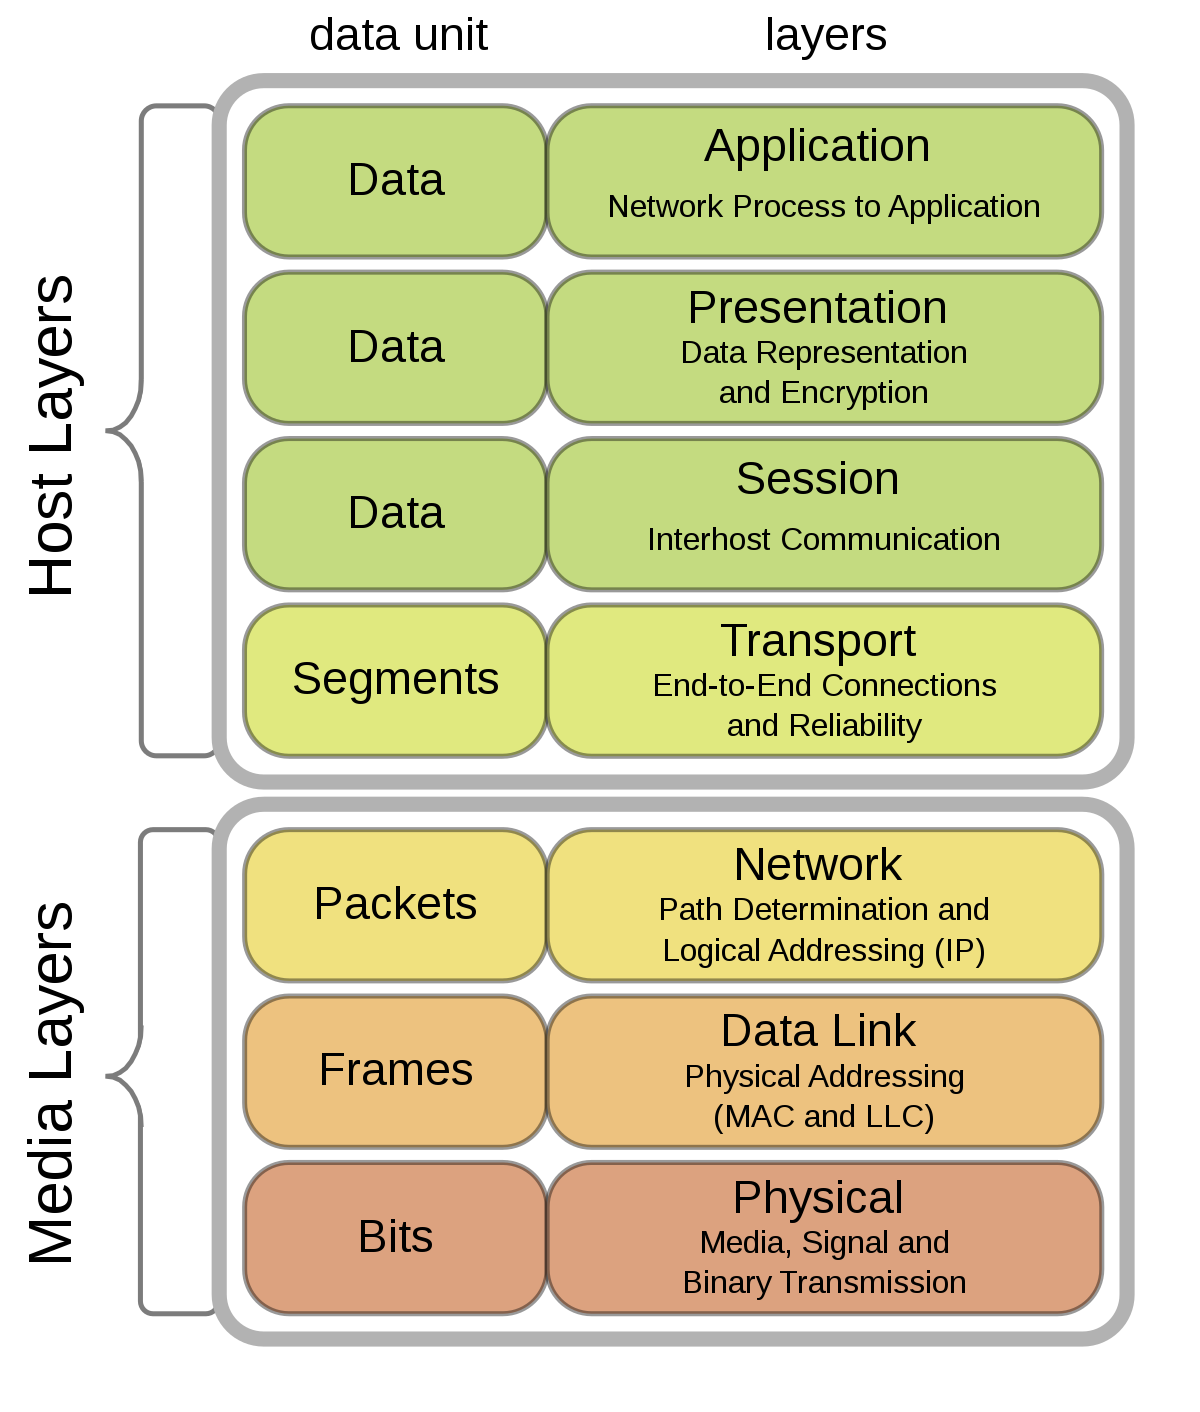
\includegraphics[scale=0.25]{images/OSI.png}
        \end{center}
        
        Ogni strato definisce un insieme di funzioni che si occupano di aspetti diversi della trasmissione dei dati. Più strati possono essere raggrupppati. I processi su due nodi che comunicano a un dato strato sono detti \textbf{peer}.
        
        In particolare, gli strati 1, 2 e 3 (\textit{fisico, collegamento, rete}) sono detti \textbf{Media Layers} e sono dedicati al supporto di rete. Le loro funzionalità hanno a che fare con problematiche del mezzo fisico (specifiche elettriche, connessioni fisiche, indirizzi di rete, sincronizzazione, controllo degli errori).
        
        Invece, gli strati 5, 6 e 7 (\textit{sessione, presentazione, applicazioni}) sono detti \textbf{Host Layers} e sono dedicati al supporto all'utente e permettono l'interoperabilità fra sistemi che usano software diversi fra loro. 
        
        Lo strato 4 (\textit{trasporto}) collega i due gruppi di strati appena descritti, e solitamente viene affibbiato al gruppo di Host Layers.
        
        \vspace{3mm}
        
        Tutti gli strati degli Host Layers sono implementati a livello software, in genere nel sistema operativo. Gli strati dei Media Layers sono ibridi, e cioè implementati a livello sia software che hardware, eccetto che per lo strato fisico, il quale è implementato esclusivamente a livello hardware.
        
        Riprendendo il concetto esposto prima per il quale la flessibilità di un modello si concretizza nella capacità di non usare tutti i layer, si prenda in esame un generico \textit{router}: un dispositivo del genere (talvolta chiamato \textbf{nodo intermedio}), che permette a più sottoreti di interfacciarsi fra di loro, ha necessità solo di uno strato fisico, uno strato di collegamento e uno strato di rete per poter funzionare.
        
        Il modello ISO-OSI è dunque \textbf{modulare}, proprio perché la stratificazione viene impiegata dinamicamente in base alle necessità.
        
        Si osservi che fra due nodi, lo strato \(n\) di un nodo comunica con il corrispondente strato \(n\) di un altro nodo. 
        
        I processi su due nodi che comunicano a un dato strato sono detti \textbf{peer}. Tale comunicazione avviene per mezzo di \textbf{interfacce}. L'implementazione interna dello strato è irrilevante, a patto che fornisca l'esatta interfaccia ad ambo i nodi.
    
    \subsubsection{Trasmissione stratificata dei dati}
    
        \textbf{I dati vengono trasmessi di strato in strato}, a partire da quello più in alto del mittente, per finire in quello più in basso, per poi rientrare dal livello più in basso del destinatario e concludere il suo viaggio al livello più in alto.
        
        \vspace{3mm}
        
        Il passaggio da strato fisico del mittente a strato fisico del destinatario avviene chiaramente tramite un mezzo di comunicazione (bus, hub, cavo, rif. \textit{topologia delle reti}).
        
        \vspace{3mm}
        
        L'utente invia il messaggio tramite lo strato applicativo, magari tramite il Web, un client FTP o qualsiasi altra interfaccia.
        
        \vspace{3mm}
        
        Il viaggio di un pacchetto dati è più o meno sintetizzabile come segue:
        
        \vspace{3mm}
        
        \(>\) Application (Mittente) 
        
        \(>\) [..] 
        
        \(>\) Physical (Mittente) 
        
        \(>\) Physical (Destinatario) 
        
        \(>\) [..] 
        
        \(>\) Application (Destinatario)
        
        \vspace{3mm}
        
        \textbf{Quello che in effetti succede è che ogni strato aggiunge delle informazioni che vengono ereditate dagli strati successivi.}
        
        L'utente invia un dato, un informazione, un messaggio, qualsiasi cosa tramite l'\textbf{Application Layer}. Tale messaggio è indicato come \textit{D7}. Quando è ancora nell'Application Layer, \textit{D7} viene accodato ad un header, cioè un'intestazione contenente svariate informazioni sulla trasmissione dei dati, denotato come \textit{H7}. Il Presentation Layer riceverà un dato del tipo "\textit{H7-D7}". 
        
        \vspace{3mm}
        
        A questo punto, il \textbf{Presentation Layer} accorperà insieme \textit{H7-D7} in un unico, grande, \textit{D6}. Infine, \textit{D6} viene accodato ad un ulteriore header, denotato con \textit{H6}. 
        
        \vspace{3mm}
        
        Il dato \textit{H6-D6} è chiaramente più grande di \textit{H7-D7}. Questo processo viene ripetuto fino allo strato di collegamento. 
        
        \vspace{3mm}
        
        Il \textbf{Data Link Layer}, oltre ad aggiungere il proprio header e accorpare i dati precedenti, piazzerà in coda anche un trailer \textit{T2}, dedicato al controllo degli errori. 
        
        \vspace{3mm}
        
        Il \textbf{Physical Layer}, dunque, riceverà \textit{
        H2-D2-T2}, e il loro contenuto verrà tradotto in binario e trasmesso, tramite un mezzo di comunicazione, al destinatario.
        
        \vspace{3mm}
        
        \textbf{Osserviamo che ad ogni passaggio si ha un pacchetto differente.} Un \textit{pacchetto}, in questo caso, è l'insieme costituito da header, body e trailer.
        
        \vspace{3mm}
        
        Quando il pacchetto arriva nel Phyisical Layer del destinatario, nella sua risalita viene mano a mano smontato. Ogni strato accederà all'header, leggerà delle informazioni, rimuoverà l'headear e scorporerà il body per recuperare l'header successivo. Analogamente per il trailer all'accesso al Data Link Layer.
        
        \vspace{3mm}
        
        I pacchetti vengono incapsulati senza conoscere alcuna informazione relativa all'header dello strato superiore. Il livello \(n-1\) non sa assolutamente niente dell'intestazione del livello \(n\), ma considera tutto il blocco come una singola unità di dati. L'accorpamento descritto fino ad ora è, difatto, \textbf{un passaggio implicito e automatico}.
    
    \subsubsection{Sintesi del funzionamento degli strati}
    
        Questa sottosezione vuole solo elencare in modo molto sintetico le funzionalità principale degli strati del modello ISO-OSI. Per maggiori dettagli, consultare la rispettiva sezione in questo blocco di appunti.
    
        \subsubsubsection{Physical Layer}
        
            Lo \textit{strato fisico} si preoccupa di trasmettere i singoli bit sul mezzo trasmissivo da un nodo ad un altro. Questo significa che lo strato fisico controlla le funzioni richieste per convertire una sequenza di bit negli opportuni segnali da spedire sul mezzo di collegamento. 
            
            \vspace{3mm}
            
            In particolare, lo strato fisico definisce la velocità con cui i segnali vanno spediti; in che modo i bit devono essere sincronizzati per essere letti correttamente dal destinatario; come vanno rappresentati i bit e codificati in segnali; come definire il tipo di mezzo trasmissivo impiegato; di che tipo è la comunicazione (simplex, half-duplex, duplex); di che tipo è la topologia della rete; com'è configurato il collegamento fra i nodi (punto-punto, multipunto).
        
        \subsubsubsection{Data Link Layer}
        
            Lo \textit{strato di collegamento} si occupa della trasmissione affidabile di pacchetti di dati fra un nodo ed il successivo. 
            
            \vspace{3mm}
            
            Per svolgere questo compito, lo strato di collegamento ha molteplici responsabilità: \textbf{framing} (dividere il flusso di bit che arriva dallo strato inferiore in frame da essere spediti allo strato superiore), indirizzi fisici (aggiungere un'intestazione contenente l'indirizzo fisico del destinatario), controllo del flusso (meccanismi per evitare il sovraccarico nel caso in cui il destinatario può ricevere i bit solo a velocità minore rispetto alla velocità del mittente), controllo degli errori (frame duplicati, frame danneggiati), controllo dell'accesso multiplo (nel caso di collegamenti multipunto, lo strato controlla quale nodo ha accesso al mezzo di trasmissione) e così via.
            
            \vspace{3mm}
            
            Lo strato di collegamento usa gli \textbf{indirizzi fisici} (MAC) delle interfacce di rete per far comunicare due nodi sulla stessa rete.
            
            \vspace{3mm}
            
            La \textit{consegna dei frame}, detta \textbf{hop}, avviene fra due nodi successivi. Tale consegna può essere diretta o indiretta. Nel caso di una consegna indiretta, e cioè a più passaggi, i frame conterranno gli stessi dati, ma headers e trailers varieranno per ogni spedizione. 
            
            La consegna indiretta avviene quando la comunicazione dev'essere stabilita fra nodi su reti diverse. Si noti, infine, che la consegna indiretta è concettualmente una sequenza di consegne dirette.
        
        \subsubsubsection{Network Layer}
        
            Lo \textit{strato di rete} si occupa della consegna di pacchetti da un \textbf{nodo mittente} ad un \textbf{nodo destinatario}, attraversando uno o più nodi intermedi. 
            
            Se due nodi sono sulla stessa rete, non avranno bisogno dello strato di rete per comunicare; altresì, fintanto che è necessario instradare il percorso del pacchetto da un nodo A ad un nodo B tramite dei router, allora lo strato di rete è indispensabile.
            
            \vspace{3mm}
            
            Se per raggiungere la destinazione si devono attraversare più nodi, si parla di \textit{consegna indiretta}.
            
            \vspace{3mm}
            
            Questo strato utilizza gli \textbf{indirizzi logici} (IP), composto da 32 bit e rappresentato in notazione decimale puntata, per identificare i nodi da raggiungere. 
            
            Ciò significa che, mentre nello strato di collegamento si ha a che fare con un indirizzamento fisico, nello strato di rete si affronta, invece, un indirizzamento puramente logico, e cioè che non dipende da alcuna componente fisica.
            
            \vspace{3mm}
            
            Il compito principale dello strato di rete è il \textbf{routing} (instradamento). Quando più reti sono connesse fra di loro per creare una interrete, i nodi che intercorrono fra le singole reti (e cioè i nodi intermedi, dunque i router) hanno il compito, appunto, di instradare i pacchetti verso la destinazione finale. 
            
            \textbf{Il pacchetto originale viene suddiviso in pacchetti più piccoli}, detti \textit{segmenti}, che possono seguire percorsi diversi. Al raggiungimento del nodo destinataro, il pacchetto viene riassemblato.
        
        \subsubsubsection{Transport Layer}
        
            Formalmente, lo \textit{strato di trasporto} si occupa della consegna di un messaggio da un processo mittente ad un processo destinatario. 
            
            \vspace{3mm}
            
            Si ponga il caso di avere aperti sul proprio computer Microsoft Teams, Google Chrome e Telegram. Quando mi connetto ad una conferenza su Teams sto chiaramente inviando e ricevendo costantemente dati relativi alle immagini, al suono e via dicendo. Ma quando questi dati arrivano, come fanno a capire che devono essere relazionati ed associati a Teams e non, ad esempio, Chrome? Sia Teams che Chrome condividono lo stesso canale di comunicazione (la propria rete), ma i dati che invio e ricevo tramite Teams devono finire su Teams, e non su Chrome o qualsiasi altro applicativo che usa la mia connedssione.
            
            \vspace{3mm}
            
            In effetti, lo stato di trasporto si occupa proprio di determinare il programma (inteso come processo) al quale devono essere effettivamente inviati i pacchetti dati. L'informazione che mi permette di capire a quale proceso inviare i dati è la porta di rete (es. localhost:\textit{8080}), motivo per cui è necessario aggiungere un ulteriore tipo di indirizzamento, contenuto nell'intestazione pervenuta dallo stato di sessione.
            
            \vspace{3mm}
            
            Questo indirizzamento è chiamato \textbf{indirizzamento dei processi} ed è rappresentato dai numeri di porta.
            
            \vspace{3mm}
            
            Inoltre, lo stato di trasporto si occupa della segmentazione del riassemblaggio dei pacchetti, e del controllo della connessione. Lo stato di trasporto, infatti, offre un servizio che può essere con o senza connessione. 
            
            In una \textbf{comunicazione senza connessione}, i dati vengono spediti in pacchetti indipendenti l'uno dall'altro; invece, in una \textbf{comunicazione con connessione}, lo strato di trasporto del mittente crea una connessione con lo stato di trasporto del destinatario prima di trasferire pacchetti contenenti i dati veri e propri. Inoltre, fra i due vi è la differenza che, rispettivamente, i pacchetti eseguono lo stesso percorso, ed eseguono percorsi differenti.
            
            Infine, lo stato di trasporto controlla, fra i processi terminali (mittente e destinatario), la velocità di trasmissione dei dati, nonché eventuali errori nell'intero processo. Questa caratteristica dello strato di trasporto è denominata "controllo del flusso".
        
        \subsubsubsection{Session Layer}
        
            Lo \textit{strato di sessione} si occupa del controllo di dialogo e della sincronizzazione. Stabilisce, mantiene e sincronizza l'interazione fra i sistemi che comunicano. Questo strato, seppur concettualmente semplice, è fondamentale: permette, infatti, a due sistemi \textit{\textbf{diversi}} di comunicare.
        
        \subsubsubsection{Presentation Layer}
        
            Lo \textit{strato di presentazione} si occupa della sintassi e della semantica dell'informazione trasmessa, dunque cifratura, compressione e traduzione di dati in bit da trasmettere.
        
        \subsubsubsection{Application Layer}
        
            Lo \textit{strato di applicazione} fornisce i servizi di rete all'utente finale. Servizi di posta, World Wide Web, accesso a file remoti, gestione condivisa di database e tanto altro.
            
    \subsection{Accenni alla Suite TCP/IP}
        L'ISO-OSI è un modello di riferimento, nel senso che si suppone che i produttori di hardware e software seguino gli standard proposti per sviluppare i propri servizi. La \textbf{suite TCP/IP} è stata sviluppata quando il modello OSI non era ancora diventato uno standard, motivo per cui sorgono delle disambiguità fra i due. 
    
        \begin{center}
            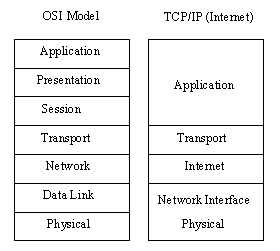
\includegraphics{images/TCP.png}
        \end{center}
    
        La suite TCP/IP permette il funzionamento di Internet. Si ispira all'ISO-OSI e ha una stratificazione a livelli. Ha 5 strati (4 se si accorpano lo strato fisico e quello di collegamento). Il TCP/IP non specifica, né per lo strato fisico, né per lo strato di collegamento, alcun protocollo. Si può usare qualsiasi protocollo previsto dall'hardware di rete. 
    
    \subsubsection{Funzionamento e tipi di indirizzamento}
        Il protocollo che adempie alle funzionalità dello strato di rete è l'\textbf{Internet Protocol} (IP), che usa l'indirizzamento logico per la consegna di pacchetti da un nodo all'altro (datagram). Lo strato di rete non permette una consegna affidabile dei dati perché i datagram possono seguire strade diverse e quindi arrivare alla destinazione in ordine diverso da quello di spedizione, o addiritura duplicarsi o venire persi. Questo servizio di consegna è chiamato "\textit{best-effort}".
        L'IP "\textit{fa del suo meglio}", senza però offrire garanzia alcuna. Ulteriori protocolli utilizzati nello strato di rete sono \textit{ARP} e \textit{RARP} (risoluzone indirizzi), \textit{ICMP} (gestione degli errori) e \textit{IGMP} (trasmissione simultanea).
    
        \vspace{3mm}
    
        Lo stato di trasporto utilizza i protocolli \textit{UDP} (senza garanzie di consegna, implementata per necessità di celerità), \textit{TCP} (trasmissione affidabile) e \textit{SCTP} (per dati multimediali). L'UDP viene adoperato, ad esempio, per gli streaming su Teams: perdere un pacchetto in una conferenza non è chissà che problema, ma perdere un pacchetto durante una transazione bancaria lo è eccome. Per la transazione bancaria verrebbe utilizzato il TCP.
    
        \vspace{3mm}
    
        Lo strato applicativo, che include gli strati di presentazione e di sessione, si rifa in toto all'ISO-OSI. I "protocolli" in questo caso coincidono con i "programmi" utilizzati (posta elettronica, Web, etc).
    
        \vspace{3mm}
    
        \begin{center}
            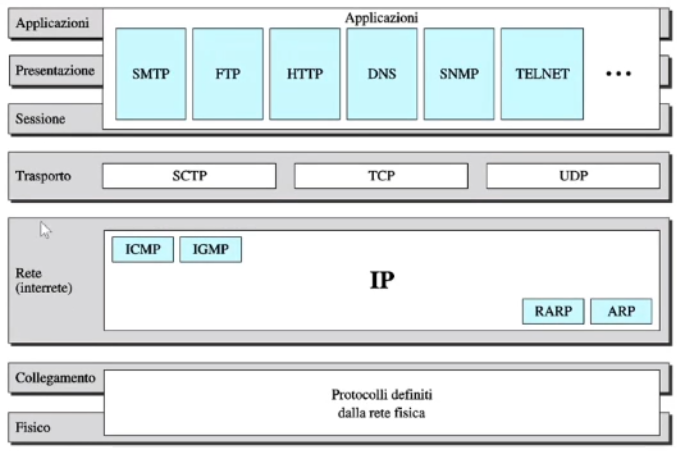
\includegraphics[scale=0.5]{images/TCP-Synth.png}
        \end{center}
    
        \vspace{3mm}
    
        Nella suite TCP/IP vengono impiegati quattro tipi di indirizzamento:
    
        \begin{itemize}
            \item 
                \textbf{Indirizzi fisici} (strato fisico e di collegamento), rappresentato dal MAC Address. E' cablato all'interno della scheda di rete, è una sequenza di 6 byte trascritti nell'interfaccia di rete.
            
            \item
                \textbf{Indirizzi logici} (strato di rete), rappresentato dall'IP Address. E' una sequenza di 4 byte in notazione decimale puntata. Ogni computer connesso ad Internet ha un indirizzo IP.
            
            \item
                \textbf{Indirizzi di porta} (strato di trasporto), rappresentato dai numeri di porta. Gli indirizzi IP e MAC sono necessari per far arrivare i dati al destinatario; tuttavia, su un singolo computer possono essere in esecuzione contemporaneamente più programmi: l'indirizzo di porta ci permette di determinare a quale programma inviare i dati. Le porte sono a 2 byte.
            
            \item
                \textbf{Indirizzi specifici} (strati applicativi), rappresentati da vari indirizzi, come l'indirizzo email.
        \end{itemize}

        Le porte più note sono la porta SSH (22) e la porta dei web server (80).
